\documentclass{article}
\usepackage{graphicx}
\usepackage{algorithm}
\usepackage[noend]{algorithmic}
\usepackage{subfigure}
\usepackage{amssymb, amsmath, graphicx, charter, latexsym}
\usepackage{layouts}
\usepackage[letterpaper]{geometry}
\usepackage{enumerate}
\usepackage{epstopdf}
\usepackage{ragged2e}
%\usepackage{times}
\usepackage{mathtools}
%\usepackage[scaled]{helvet}
\usepackage{mathptmx}
\usepackage{verbatim}
\usepackage{listings}
\usepackage{siunitx}
\usepackage{booktabs}
\usepackage{array}
\DeclareMathOperator*{\argmin}{arg\,min}
\DeclareMathOperator*{\argmax}{arg\,max}
\newcolumntype{P}[1]{>{\centering\arraybackslash}p{#1}}

\lstset{
basicstyle=\ttfamily,
}
\lstMakeShortInline|

\begin{document}

\title{\bfseries ECEN 689 -- Real-Time Wireless Networks: Project 3\\
S-WiFi: Smart Scheduling with Point Coordination Function for WiFi Uplink Transmissions}
\date{Due on 5/6}
\author{%
Ping-Chun Hsieh\\
\texttt{lleyfede@tamu.edu}
\and
Tao Zhao\\
\texttt{alick@tamu.edu}
\and
Dongni Han\\
\texttt{handongni2015@tamu.edu}
}
\maketitle

\section*{Terminology}

In our report, we use AP or ``server'' to denote the WiFi access point, and ``client'' to denote the terminal device such as a mobile phone, a tablet, and so on. Throughout our simulation, we let node $0$ be the server, and the other nodes be the clients. The basic time unit for packet transmission is called \emph{slot}, which should be greater than a round-trip time (RTT). For real-time traffic, we group an integer number (denoted by $T$) of slots into an \emph{interval}, which is the relative deadline of the packets.

\section{Background}
\subsection{System Model}
We consider a wireless network of one AP and $N$ clients, where $N\ge1$. We consider uplink transmission with point coordination function (PCF) with real-time traffic. For uplink transmission, packets are generated by each client $n$ in the beginning of each interval. In each interval, the number of packets generated by client $n$, denoted by $X_n$, follows a uniform distribution in the range of [$U_{min}$, $U_{max}$]. In PCF mode, AP polls at most one client per slot and it has full control over channel allocation. In the beginning of each interval, each client generates a random number of packets and waits for channel access that is fully controlled by the AP. Since the packets are generated and queued on the client's side, the AP needs to collect the queue information of the clients to make scheduling decisions.

\subsection{Baseline Policy}
Under the baseline policy, the AP first collects the queue information by polling each client one by one for the number of data packets it generates ($X_n$). After all clients are polled, the AP knows the number of packets at each client. Next, the AP uses the Max-Weight policy to schedule one of the clients in each time slot for actual data transmission. 

The major issue in the baseline policy is that there is no data transmission in the polling phase. As a result, channel utilization for data packets can be very low. Moreover, the channel utilization is especially low with large network size or poor wireless channels since the AP ends up spending most of the time on polling queue information.

\section{Smart Policy}

We introduce three different features to improve network performance with real-time traffic.
\subsection{Selective Polling}
The first feature is selective polling. In each interval, the AP only polls the queue information of a subset of $n \le N $ clients. By properly choosing $n$, the AP avoids spending too much time on polling queue information while collecting enough queue information for scheduling. The process of determining the optimal $n$ includes the following three steps:
\begin{enumerate}
\item Sort clients by channel reliabilities $p_1 \geq p_2 \geq \dots \geq p_N$
\item Estimated throughput: $\hat{R}_n = \min\{n\frac{U_{min}+U_{max}}{2}, (T-\sum_{i=1}^{n}\frac{1}{p_i})\frac{\sum_{i=1}^{n}p_i}{n} \}$
\item Find the optimum $n^* = \argmax_{n} \hat{R}_n$
\end{enumerate}
Step 1 allows us to look at only the first $n$ clients in step 2. In step 2, $(T-\sum_{i=1}^{n}\frac{1}{p_i})$ serves as an estimate of the average number of slots available for data packets and $(\frac{\sum_{i=1}^{n}p_i}{n})$ is the average channel reliability of this subset of clients.
In selecting clients, we apply random permutation for better fairness by using Knuth shuffle algorithm. When all of the selected clients are served completely, we consider the  remaining clients by serving them one by one.
[NEED TO ADD MORE IMPLEMENTATION DETAILS]

\subsection{Piggybacked Queue Length}

The polling overhead can be greatly mitigated by allowing piggybacked queue information. When a client receives a polling message, it replies with its queue length $X_n$ as well as the first data message (if there is any) in one packet to the AP. Hence, all slots become effectively available for data transmission. Consequently, when this feature is combined with selective polling, the estimated throughput used in selective polling should be modified as $\hat{R}_n = \min \{n\frac{U_{min}+U_{max}}{2}, T \frac{\sum_{i=1}^{n}p_i}{n} \}$. 

To implement this feature in ns-2, we introduce two new packet types: \lstinline|SWiFi_PKT_POLL_PGBK| for the AP and \lstinline|SWiFi_PKT_PGBK_UL| for the clients. The queue information is maintained in the header of \lstinline|SWiFi_PKT_PGBK_UL| packets. This feature is designed to be enabled/disabled by one boolean variable.

\subsection{Retry Limit for Polling}

Consider a network where there is one client with zero channel reliability. Under the baseline policy, the AP will keep polling the queue information of that unconnected client indefinitely and end up producing zero data throughput. As a countermeasrue, retry limit for polling can prevent the AP from spending too much time on polling clients with poor channels. 
To implement this feature, we choose to disable the built-in retry function of 802.11 MAC and handle retransmission completely in the application layer. This allows us to have full control over the timing of retransmissions. We introduce a variable \lstinline|num_retry_| to keep track of the number of retries. When the AP starts polling a new client, \lstinline|num_retry_| is set to 0. \lstinline|num_retry_| increases by 1 after each polling retry. If the retry limit is reached, the AP then starts polling the next client regardless of the result of the last transmission. 

\subsection{Smart Policy}
Our smart policy combines selective polling, piggybacked queue length, and retry limit for polling to handle the polling issue in the baseline policy. For better modularity, our design allows users to enable the above three features independently. In Tcl domain, we use binary digits to represent different types of policies. All combinations of the three features are shown in Table \ref{Policy Types}. 

\begin{table}[htbp]
   \centering
   \caption{Policy types and binary representation.}
   \label{Policy Types}
   \begin{tabular}{| P{4cm} | P{3.5cm} |}
       \hline
       Policy Types   &  Binary representation\\   \hline
       Baseline &  000\\ \hline
       Selective & 001\\ \hline
       Piggyback & 010\\ \hline
       Selective + Piggyback & 011\\ \hline
       Retry Limit  &100\\ \hline
       Selective+ Retry Limit & 101\\ \hline
       Piggyback + Retry Limit & 110\\ \hline
       Smart &  111\\
       \hline
   \end{tabular}
\label{table: policy}
\end{table} 

%\begin{enumerate}
%\item Select a subset of clients to poll $X_n$.
%\item AP polls clients in expect of piggybacking reply.
%\item AP repeats polling a client for limited times.
%\end{enumerate}

%\section{Implementation in NS-2}
%\label{section: ns2}


\section{Simulation Results}
\subsection{Simulation Setup}
\label{section: simulation: setup}
Throughout the simulation, we consider a network of one AP and 5 clients unless stated otherwise. We use the shadowing module as the wireless channel. The parameters of the channel are shown in Table \ref{table: channel}. The transmitter power is $\SI{1}{W}$, and the channel reliability is varied by changing the distance between the AP and the clients. 

\begin{table}[htbp]
\centering
    \caption{Parameters of the wireless channel.}
    \vspace{2mm}
    \begin{tabular}{ | l | l | }
    \hline
    Item & Value \\ \hline
    Path loss exponent & 2.0  \\ \hline
    Shadowing deviation & \SI{4.0}{dB} \\ \hline
    Reference distance & \SI{1.0}{m} \\
    \hline
\end{tabular}
\label{table: channel}
\end{table}

\begin{table}[htbp]
\centering
\caption{Parameters of the 802.11b MAC.}
    \vspace{2mm}
    \begin{tabular}{ | l | l | }
    \hline
    Item & Value \\ \hline
    Data rate & \SI{11}{Mb/s}  \\ \hline
    Basic rate & \SI{1}{Mb/s}  \\ \hline
    PLCP data rate & \SI{1}{Mb/s}  \\ \hline 
    Preamble length & \SI{144}{bits} \\ \hline
    Slot time & \SI{20}{\mu s} \\ \hline
    SIFS & \SI{10}{\mu s} \\
    \hline
\end{tabular}
\label{table: mac}
\end{table}

For the medium access control (MAC) layer, we use the 802.11 MAC module built in ns-2 and the key parameters are summarized in Table \ref{table: mac}. As mentioned earlier, we disable the automatic retransmission function of 802.11 MAC by letting \lstinline|ShortRetryLimit_| and \lstinline|LongRetryLimit_| be 0 in the Tcl script.

In the application layer, 1 time slot is chosen to be $\SI{10}{ms}$ to ensure enough margin for data transmission. The key simulation parameters are summarized in Table \ref{table: parameter}. In the fully-symmetric case, we let $p_i = p$, for any client $i$. In the asymmetric scenario, we let $p_1 = p_2 = 1$ and $p_j = p$, for $j = 3, ..., N$. We use the timely-throughput of the network as our primary performance metric to evaluate different scheduling policies.
\begin{table}[htbp]
\centering
    \caption{Simulation parameters.}
    \vspace{2mm}
    \begin{tabular}{ | l | l | }
    \hline
    Item & Value \\ \hline
    Slot time & \SI{10}{ms}  \\ \hline
    Interval length & \SI{10}{slots} \\ \hline
    $U_{\min}$ & 0 \\ \hline
    $U_{\max}$ & 2 \\ \hline
    Retry limit & 1 \\ \hline
    Simulation runs & 10 \\
    \hline
\end{tabular}
\label{table: parameter}
\end{table}

%Each interval contains 10 time slots. The number of packets generated follows uniform distribution in the range of $U_\text{min}=0, U_\text{max}=2$. Channel reliability $p\approx0.57$ which its distance is \SI{1000}{m}. Retry limit is one. Every 

\subsection{Performance Over Symmetric Channels}
We first evaluate the policies in the fully-symmetric scenario. Figure \ref{sim: sym: smart and baseline} shows the network timely-throughput with different channel reliabilities under the Smart policy and the baseline policy. The Smart policy achieves larger timely-throughput than the baseline policy regardless of the channel reliability. In particular, the Smart policy makes the most significant difference when the channel reliability is moderate. Moreover, the Smart policy is able to deliver all packets when $p=1$ while the baseline policy can not. This is because the baseline policy spends half of the interval on polling queue information so that there are only 5 slots left for data transmission. 

\begin{figure}[htbp]
\centering
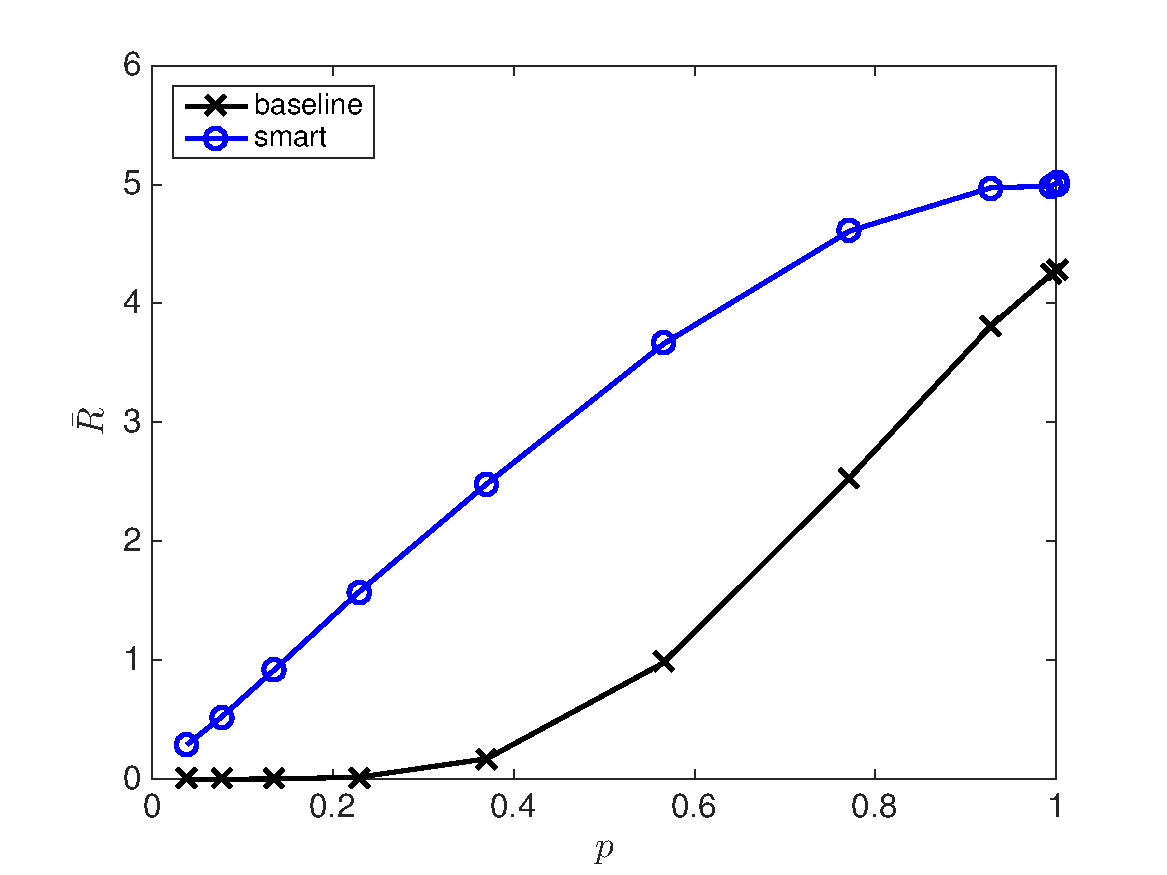
\includegraphics[scale=0.5]{R_p_sym.pdf}
\caption{Throughout versus channel reliability in the fully-symmetric scenario.}
\label{sim: sym: smart and baseline}
\end{figure}

Next, we evaluate the performance of each individual feature. Figure \ref{sim: sym: three features} shows the timely-throughput with the selective, piggyback, and the retry limit feature in the fully-symmetric case. Among the three features, the piggyback function provides the most performance gain regardless of the channel condition. The selective or the retry limit function also individually improves the network timely-throughput when the channel reliability is less than 0.8. This is because the polling overhead under the baseline policy becomes much more significant when the channel is less reliable. Figure \ref{sim: sym: combined} further shows the performance of the policies with combined features. In the symmetric scenario, the piggyback feature per se already achieves similar performance as the Smart policy. 

\begin{figure}[htbp]
\centering
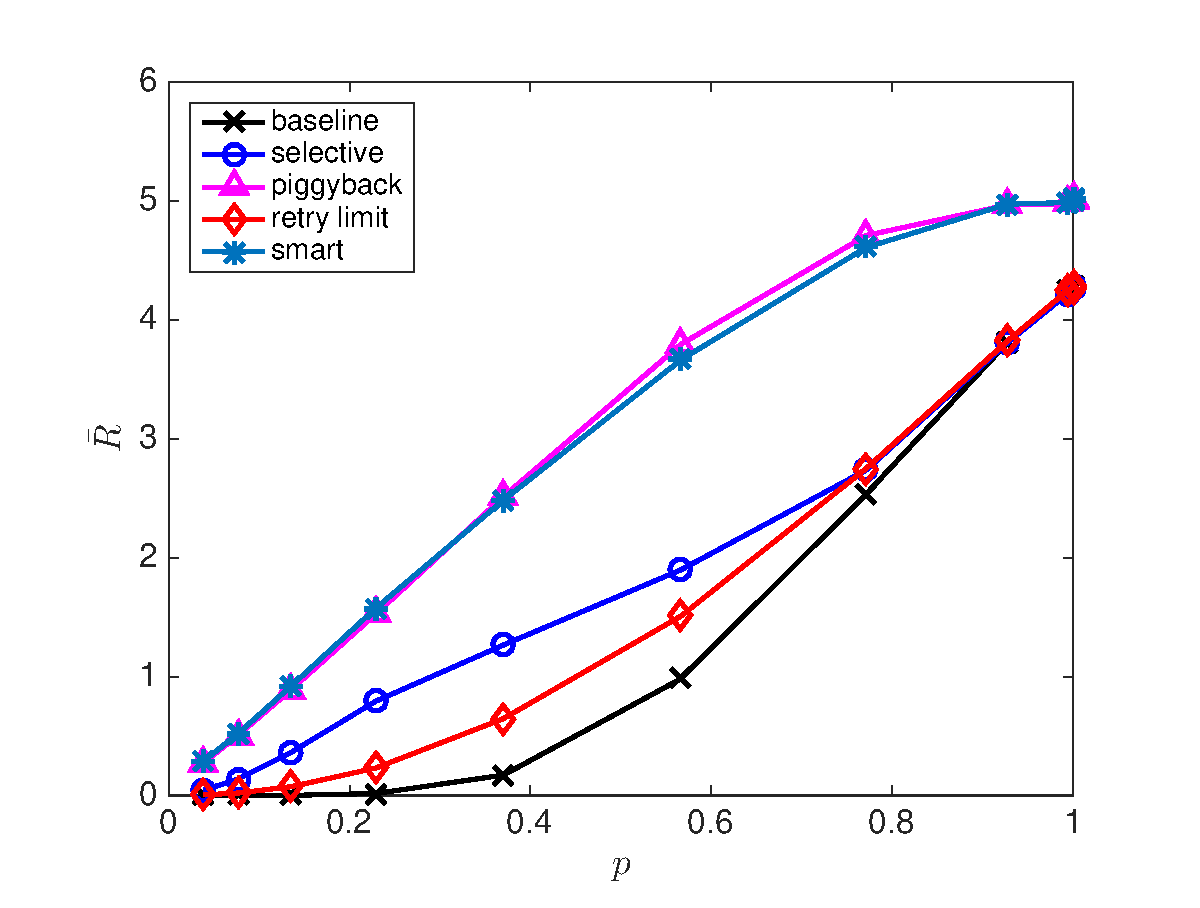
\includegraphics[scale=0.5]{3policycompare_sym.eps}
\caption{Throughout versus channel reliability in the fully-symmetric scenario: baseline, Smart, and each individual feature.}
\label{sim: sym: three features}
\end{figure}
\begin{figure}[htbp]
\centering
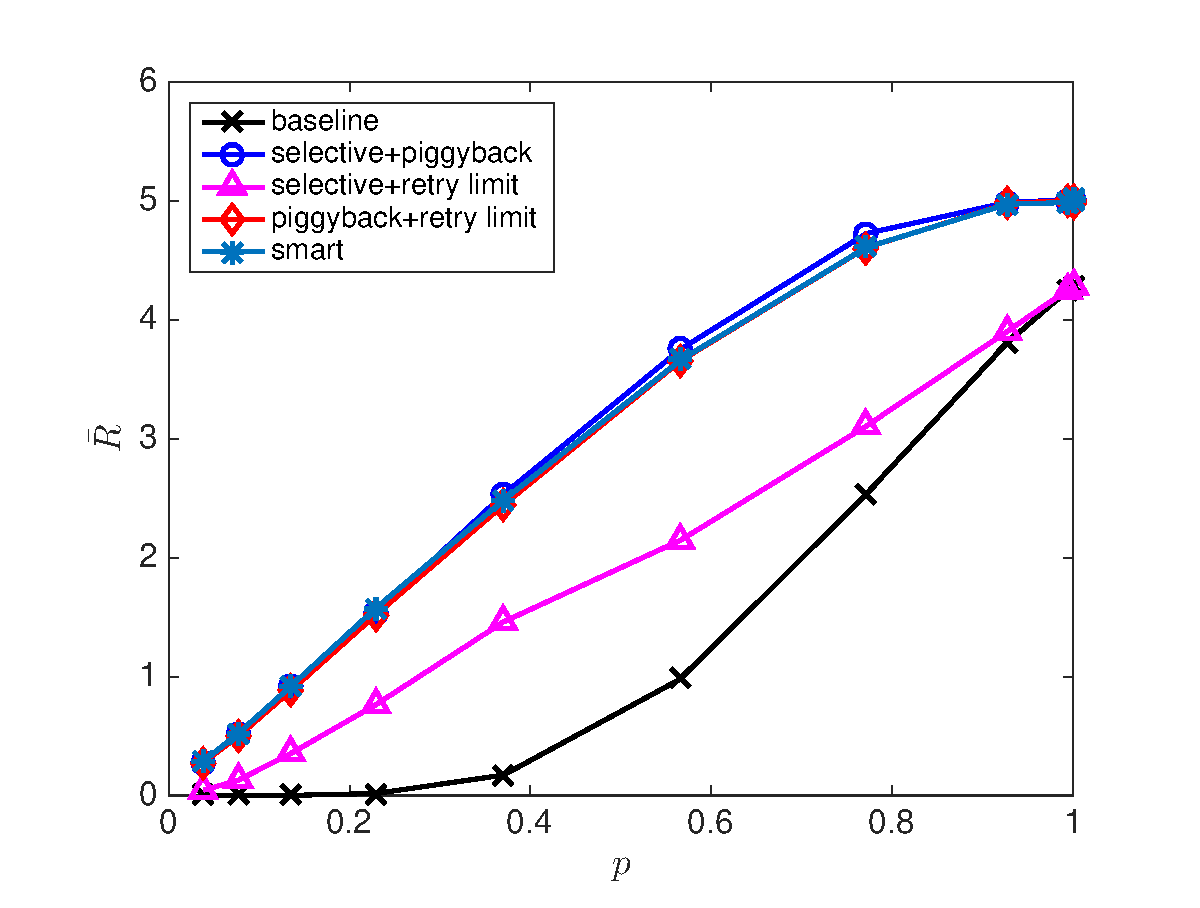
\includegraphics[scale=0.5]{sym_threecombinepolicys.eps}
\caption{Throughout versus channel reliability in the fully-symmetric scenario: baseline, Smart, and polices of combined features.}
\label{sim: sym: combined}
\end{figure}

We are also interested in the effect of network size on the overall performance. Figure \ref{sim: sym: different N} shows the total timely-throughput with different number of clients and the channel reliability $\approx 0.57$. The Smart policy performs steadily when the number of clients increases from 5 to 10. On the other hand, the baseline policy provides nearly zero timely-throughput when there are more than 8 clients. This shows that the Smart policy also achieves much better scalability.

\begin{figure}[htbp]
\centering
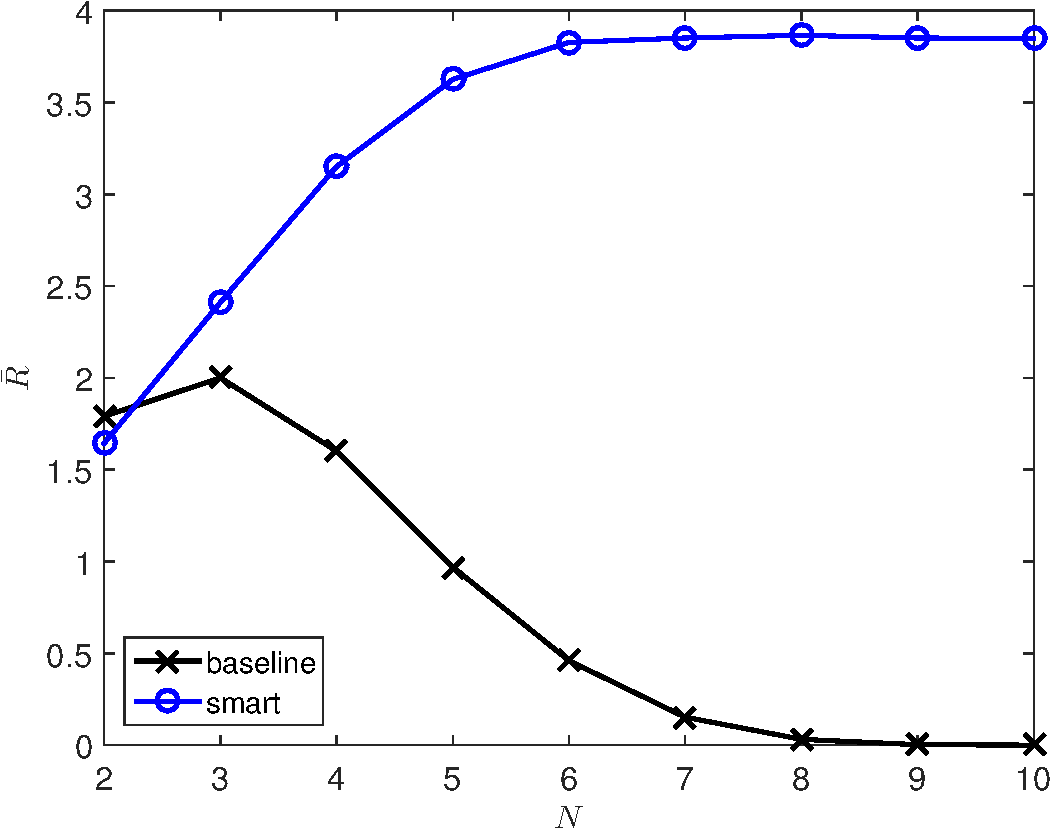
\includegraphics[scale=0.5]{R_N_sym.pdf}
\caption{Throughout versus number of clients in the fully-symmetric scenario.}
\label{sim: sym: different N}
\end{figure}

%Figure \ref{smart and baseline asym} shows Smart policy and Baseline policy under asymmetric channel. Smart policy is consistently better under asymmetric channel, especially when the channel is poor. \\

%Figure \ref{Combined Policies Under Symmetric Channel} shows Baseline, Selective + Piggyback, Selective + Retry Limit, Piggyback + Retry Limit and Smart policy under symmetric channel. Selective + Piggyback is the best and it is even better than smart policy. Smart and Piggyback + Retry Limit are equal, which implies that Piggyback and Retry Limit play vital roles among these three features. The worst combined policy is Piggyback and Retry Limit. \\

\subsection{Performance Over Asymmetric Channels}
Consider the asymmetric scenario described in Section \ref{section: simulation: setup}. We measure the total timely-throughput with different $p$.  Figure \ref{sim: asym: three features} shows the performance of the baseline policy, the Smart policy, and the policy of each individual feature. Among the three features, the piggyback function still achieves the most improvement and it is even slightly better than Smart policy when $p$ is between 0.6 and 0.8. Different from the symmetric case, the piggyback feature by itself can not achieve the same performance as the Smart policy when $p$ is fairly small. This shows that the piggyback feature is not able to prevent the AP from spending too much resource on the clients with very poor channel. On the other hand, the selective and the retry limit feature provide more performance gain when $p$ is less than 0.6. Interestingly, the retry limit function exhibits convexity in total timely-throughput when $p$ is between 0 to 0.4. This is because when $p$ is extremely small, the AP can not possibly receive the queue information from these clients and therefore does not spend any time on data transmission for the clients with very poor channel.

\begin{figure}[htbp]
\centering
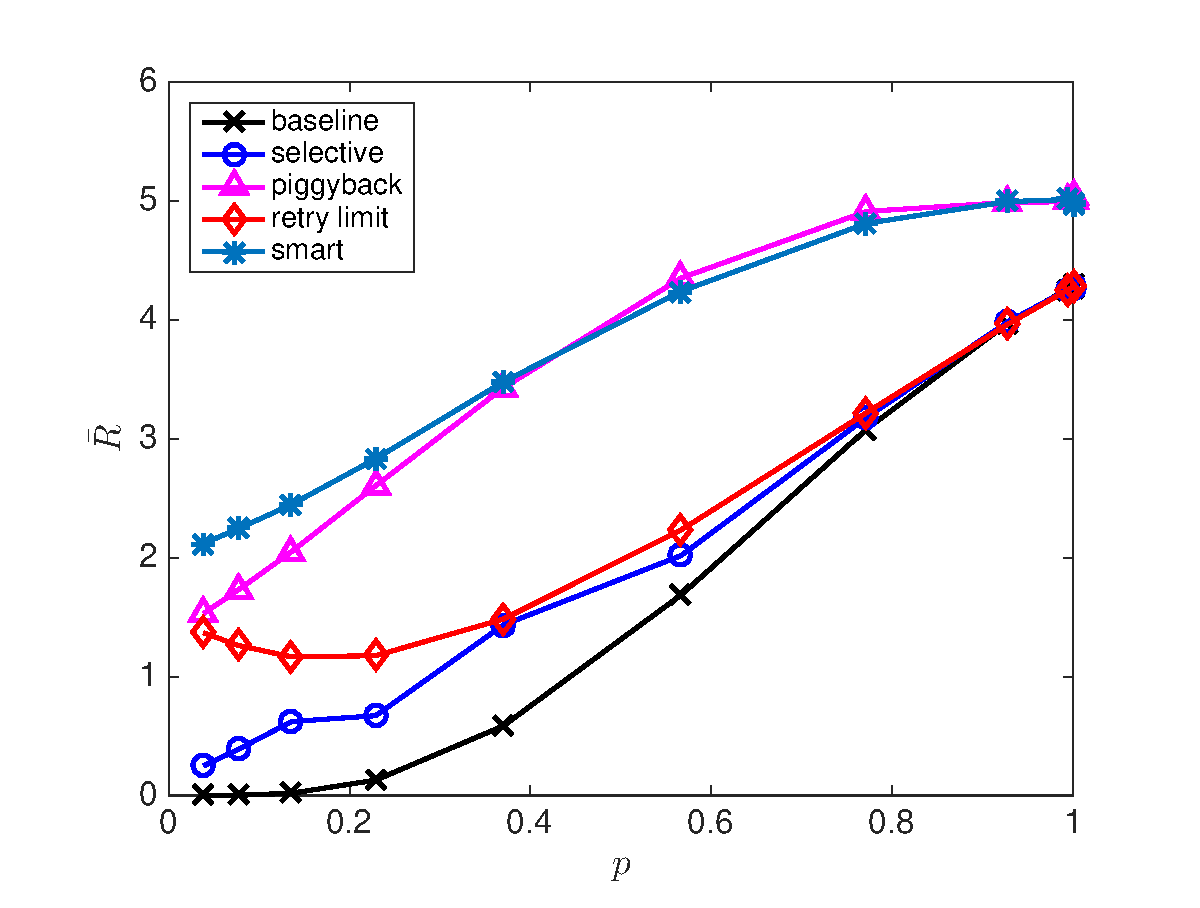
\includegraphics[scale=0.5]{3policycompare_asym.eps}
\caption{Throughout versus channel reliability in the asymmetric scenario: baseline, Smart, and each individual feature.}
\label{sim: asym: three features}
\end{figure}

Next, we evaluate the policies with two combined features, as shown in Figure \ref{sim: asym: combined}. In our asymmetric scenario, the policy with piggybacked queue length plus retry limit can achieve similar performance as the Smart policy. Therefore, it is worth studying the possible scenarios where the selective polling feature provides further timely-throughput gain in the Smart policy. 

\begin{figure}[htbp]
\centering
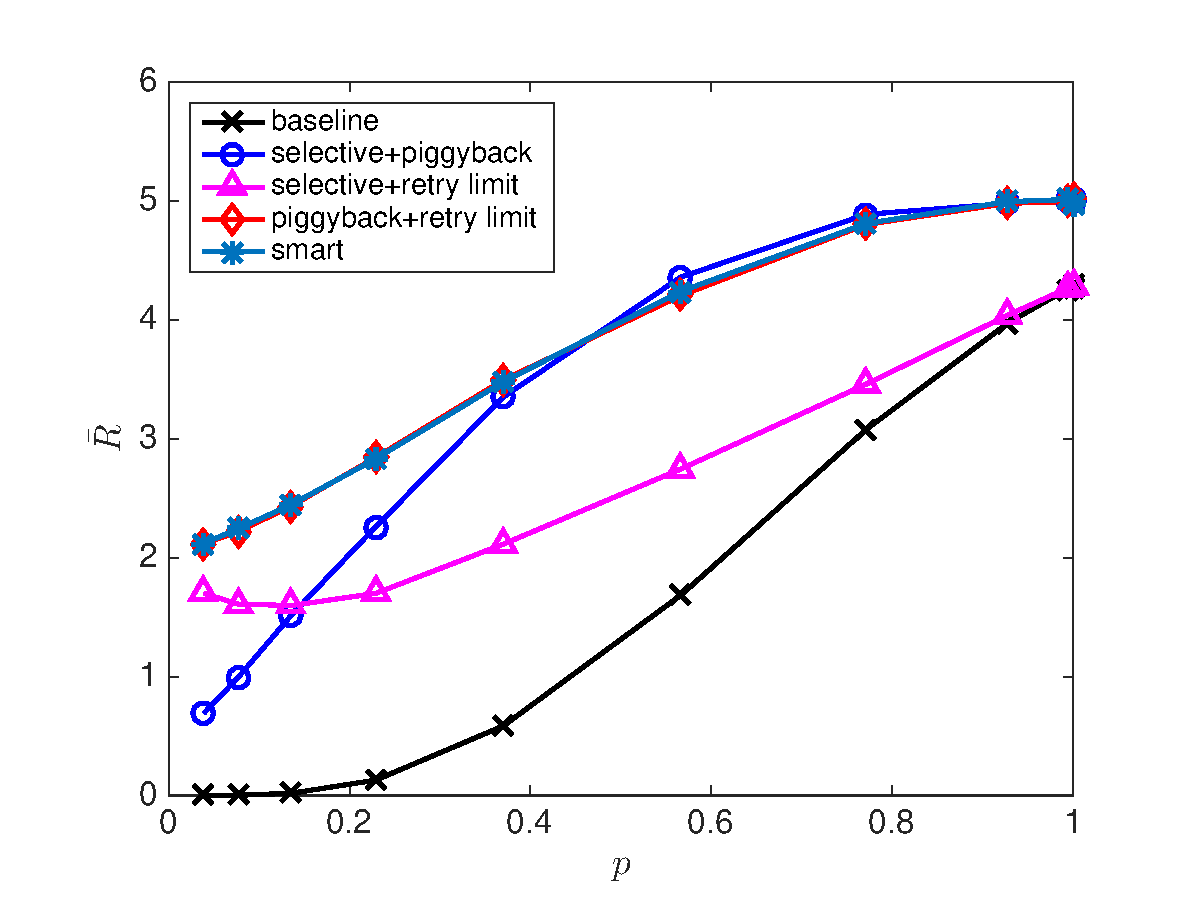
\includegraphics[scale=0.5]{asym_threecombinepolicys.eps}
\caption{Throughout versus channel reliability in the asymmetric scenario: baseline, Smart, and polices of combined features.}
\label{sim: asym: combined}
\end{figure}

%Figure \ref{Combined Policies Under Asymmetric Channel} shows Baseline, Selective + Piggyback, Selective + Retry Limit, Piggyback + Retry Limit and Smart policy under asymmetric channel. When channel reliability $p$ is smaller than 0.15, Piggyback and Retry Limit are the same. Then Selective + Retry Limit is better than Selective + Piggyback. However, Selective + Piggyback becomes better than Selective + Retry Limit when channel reliability $p$ is larger than 0.15. When channel reliability $p$ is larger than 0.5, Selective + Piggyback is the best. When channel reliability $p=1$, the system delivers all packets under Selective + Piggyback, Smart and Piggyback + Retry Limit. \\

Finally, we are also interested in the fairness of the policies. We define the utility of each client $n$ as $U_n(q_n)=\log \left(\frac{q_n}{10^{-4}}\right)$, where $q_n$ is the timely-throughput and the constant $10^{-4}$ is only an offset for ease of plotting. This utility function is widely used for achieving proportional fairness in network utility maximization problems. Figure \ref{sim: asym: utility} shows the network utility with different $p$ in the asymmetric scenario. It is clear that the Smart policy not only achieves better total timely-throughput but also maintains a certain level of fairness across the network. 

\begin{figure}[htbp]
\centering
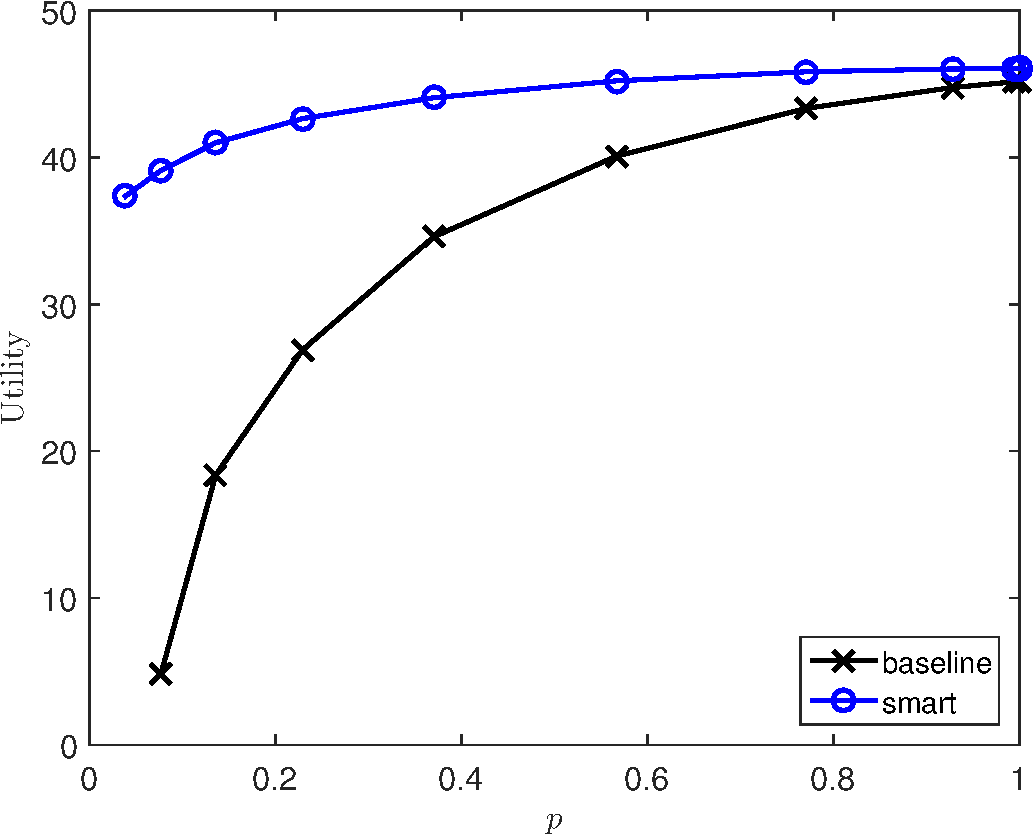
\includegraphics[scale=0.5]{U_p_asym.pdf}
\caption{Network utility versus channel reliability in the asymmetric scenario with $p\approx 0.57$.}
\label{sim: asym: utility}
\end{figure}

\section{Conclusion}
The baseline policy incurs huge overhead especially with large $N$ and poor channel. The Smart policy incorporates selective polling, piggybacking, and retry limit to improve the performance. Simulation shows the Smart policy outperforms the baseline policy in terms of timely-throughput and network utility.

\section{Appendix}
The S-WiFi project can be accessed by scanning the following QR code.
\begin{figure}[htbp]
\hspace{3mm}
\center

\includegraphics[scale=0.2]{url.pdf}
\end{figure}
\end{document}
